\chapter{أول دارة كهربائية}\label{ch:g3:first-electric-circuit}

طقّة --- فيلقي \omterm{def:g3:first-electric-circuit:bulb}{المصباح} اليدوي حزمته عبر الغرفة المظلمة. وداخل ذلك
الأنبوب البلاستيكي تعيش \omterm{def:g3:first-electric-circuit:battery}{بطارية} \omterm{def:g3:first-electric-circuit:bulb}{ومصباح} صغير وشريطان معدنيان،
يلعبون لعبة ذات قواعد صارمة. واليوم نفكّك اللعبة: فببطارية \omterm{def:g3:first-electric-circuit:bulb}{ومصباح}
وسلكين سنصنع \omterm{def:g1:light-and-shadows:source}{الضوء} بأيدينا.

\section{مصباح وبطارية وسلكان}

\begin{definition}[البطارية]\label{def:g3:first-electric-circuit:battery}
\emph{البطارية}\index{بطارية} مخزن صغير للكهرباء. ولها طرفان
مختلفان يُسمّيان \emph{قطبيها}\index{قطب}: أحدهما عليه علامة $+$
(زائد)، والآخر عليه علامة $-$ (ناقص). وكلا القطبين مهمّ ---
فالكهرباء لا تلعب إلا إذا دخل الاثنان اللعبة.
\end{definition}

\begin{definition}[المصباح]\label{def:g3:first-electric-circuit:bulb}
\emph{المصباح}\index{مصباح} لمبة صغيرة في زجاجها خيط رفيع يتوهّج
أبيض ساخنًا حين تجري فيه الكهرباء. وانظر عن قرب إلى قاعدته
المعدنية: للمصباح أيضًا موضعا تماسّ \emph{اثنان} --- الطرف في
أسفله تمامًا، والجانب المعدني من قاعدته. قطبان في \omterm{def:g3:first-electric-circuit:battery}{البطارية}،
وموضعا تماسّ في المصباح: وليس ذلك مصادفة.
\end{definition}

\begin{method}[كيف تُشعل المصباح]\label{met:g3:first-electric-circuit:light}
\omterm{def:g3:first-electric-circuit:battery}{ببطارية} واحدة \omterm{def:g3:first-electric-circuit:bulb}{ومصباح} واحد وسلكين:
\begin{enumerate}
  \item صِل سلكًا من \omterm{def:g3:first-electric-circuit:battery}{قطب} \omterm{def:g3:first-electric-circuit:battery}{البطارية} $+$ إلى طرف قاعدة \omterm{def:g3:first-electric-circuit:bulb}{المصباح}؛
  \item وصِل السلك الآخر من \omterm{def:g3:first-electric-circuit:battery}{قطب} \omterm{def:g3:first-electric-circuit:battery}{البطارية} $-$ إلى الجانب المعدني
        من القاعدة؛
  \item فيضيء \omterm{def:g3:first-electric-circuit:bulb}{المصباح} --- وتكون قد بنيت دارة!
\end{enumerate}
وإن بقي معتمًا فافحص المتّهمين المعتادين: سلك يلمس الزجاج بدل
موضع التماسّ المعدني، أو وصلة مرتخية، أو \omterm{def:g3:first-electric-circuit:battery}{بطارية} نافدة.
\end{method}

\begin{omfigure}
\begin{tikzpicture}[scale=0.85]
  \draw[thick, fill=omExo, fill opacity=0.2] (0,0.4) rectangle (1.7,3.0);
  \draw[thick] (0.55,3.0) rectangle (1.15,3.35);
  \node[font=\small] at (0.85,1.7) {بطارية};
  \node[font=\footnotesize] at (0.85,3.17) {$+$};
  \node[font=\footnotesize] at (0.85,0.65) {$-$};
  \draw[thick] (5.8,2.6) circle (0.75);
  \draw[thick] (5.45,2.0) -- (5.45,1.5) -- (6.15,1.5) -- (6.15,2.0);
  \draw[thick] (5.6,1.5) -- (5.6,1.1) (6.0,1.5) -- (6.0,1.1)
    (5.6,1.1) -- (6.0,1.1);
  \draw[thick] (5.62,2.35) .. controls (5.75,2.6) .. (5.8,2.35)
    .. controls (5.85,2.6) .. (5.98,2.35);
  \node[right, font=\small] at (6.8,2.7) {زجاج فيه الخيط المتوهّج};
  \node[right, font=\small] at (6.8,1.7) {قاعدة معدنية: تماسّ جانبي};
  \node[right, font=\small] at (6.8,1.0) {وتماسّ الطرف من تحت};
  \draw[-Stealth, omExo] (6.7,1.05) -- (5.85,1.05);
  \draw[thick, omThm] (0.85,3.35) -- (0.85,4.0) -- (5.8,4.0)
    -- (5.8,3.35);
  \draw[thick, omDef] (0.85,0.4) -- (0.85,-0.3) -- (5.8,-0.3)
    -- (5.8,1.1);
  \node[above, font=\small, omThm] at (3.3,4.05)
    {سلك: من $+$ إلى الطرف؟ لا --- بل إلى أيّ موضع تماسّ};
\end{tikzpicture}

{\small اللاعبون: \omterm{def:g3:first-electric-circuit:battery}{بطارية} \omterm{def:g3:first-electric-circuit:battery}{بقطبيها}، \omterm{def:g3:first-electric-circuit:bulb}{ومصباح} بموضعَي تماسّه،
وسلكان يصلان بينهما.}
\end{omfigure}

\begin{omfigure}
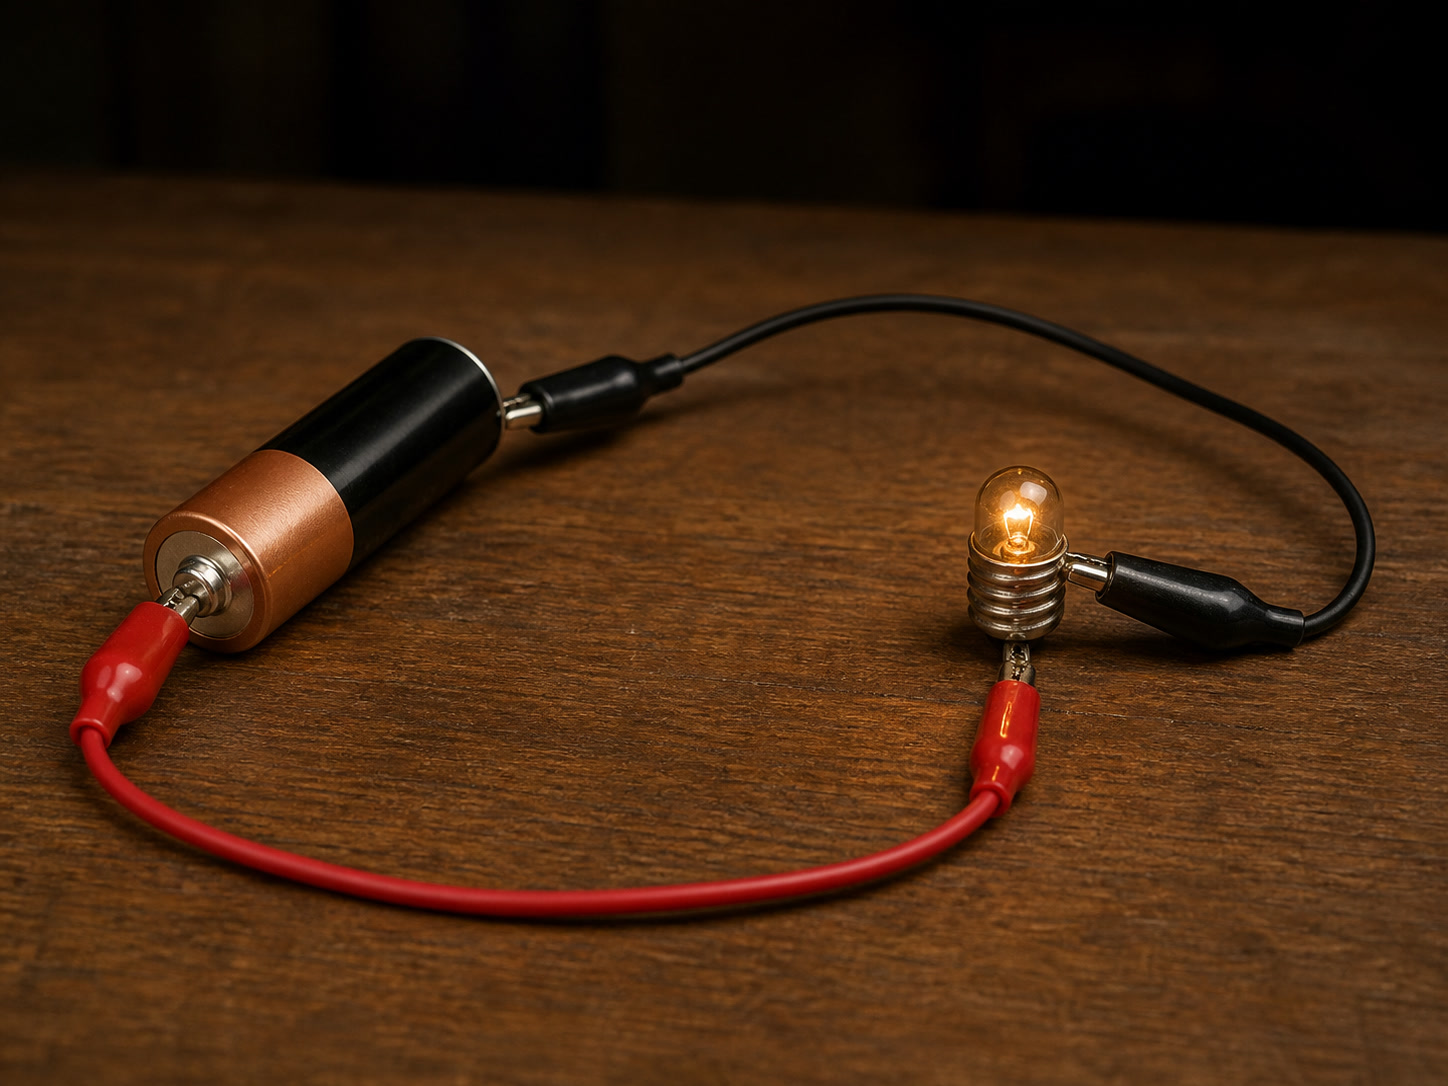
\includegraphics[width=0.5\linewidth]{images/book1/ai/g3-circuit-bulb.jpg}

{\small لحظة انغلاق الحلقة: \omterm{def:g3:first-electric-circuit:battery}{بطارية} وسلكان، فيضيء \omterm{def:g3:first-electric-circuit:bulb}{المصباح} الصغير.}
\end{omfigure}

\section{لا بدّ أن تنغلق الدارة}

\begin{definition}[الدارة الكهربائية]\label{def:g3:first-electric-circuit:circuit}
\emph{الدارة الكهربائية}\index{دارة كهربائية} حلقة كاملة تجري
فيها الكهرباء: تخرج من أحد قطبَي \omterm{def:g3:first-electric-circuit:battery}{البطارية}، وتمرّ في السلكين
\omterm{def:g3:first-electric-circuit:bulb}{والمصباح}، وتعود إلى \omterm{def:g3:first-electric-circuit:battery}{القطب} الآخر. وحين تكتمل الحلقة نقول إن الدارة
\emph{مغلقة}\index{دارة مغلقة}؛ وإن كان فيها فراغ في أي موضع
فهي \emph{مفتوحة}\index{دارة مفتوحة}.
\end{definition}

\begin{proposition}[قانون الحلقة]\label{prop:g3:first-electric-circuit:loop}
لا يضيء \omterm{def:g3:first-electric-circuit:bulb}{المصباح} إلا حين تكون \omterm{def:g3:first-electric-circuit:circuit}{الدارة مغلقة} --- حلقة واحدة غير
مقطوعة من أحد القطبين، عبر \omterm{def:g3:first-electric-circuit:bulb}{المصباح}، إلى \omterm{def:g3:first-electric-circuit:battery}{القطب} الآخر. وفراغ واحد
فقط، في أي موضع من الحلقة، يُطفئ \omterm{def:g3:first-electric-circuit:bulb}{المصباح}: فالكهرباء لا تقفز فوق
الفراغات، ولا تجري في طرق مسدودة.
\end{proposition}

\begin{example}[لماذا القطبان معًا؟]\label{ex:g3:first-electric-circuit:bothends}
صِل سلكين \emph{اثنين} من \omterm{def:g3:first-electric-circuit:battery}{قطب} \omterm{def:g3:first-electric-circuit:battery}{البطارية} $+$ إلى موضعَي تماسّ
\omterm{def:g3:first-electric-circuit:bulb}{المصباح}، واترك \omterm{def:g3:first-electric-circuit:battery}{القطب} $-$ وحده: لا شيء. وصِل سلكًا من $+$ وسلكًا
من $-$، لكن كليهما إلى طرف \omterm{def:g3:first-electric-circuit:bulb}{المصباح}: لا شيء أيضًا. ولا يضيء
\omterm{def:g3:first-electric-circuit:bulb}{المصباح} إلا حين تزور الحلقة قطبَي \omterm{def:g3:first-electric-circuit:battery}{البطارية} المختلفين
\emph{وموضعَي} تماسّ \omterm{def:g3:first-electric-circuit:bulb}{المصباح} المختلفين --- رحلةً كاملة ذهابًا
وإيابًا.
\end{example}

\begin{example}[القاطعة]\label{ex:g3:first-electric-circuit:switch}
\emph{القاطعة}\index{قاطعة} باب في الدارة: جسر معدني صغير تضعه
الطقّة (مغلقة --- فتكتمل الحلقة، \omterm{def:g1:light-and-shadows:source}{فالضوء}!) أو ترفعه (فراغ ---
فالعتمة). وزرّ \omterm{def:g3:first-electric-circuit:bulb}{المصباح} اليدوي، ومفتاح النور على الجدار، وزرّ جرس
الباب: كلها أبواب في حلقة. وتستطيع أن تصنع واحدة من مشبك غسيل
وشريط من رقاقة المطبخ مطويّ على فكّيه.
\end{example}

\begin{omfigure}
\begin{tikzpicture}[scale=0.9]
  \draw (0,0) to[battery1, l=بطارية] (0,2.4)
    to[short] (1.7,2.4)
    to[cspst, l=قاطعة مغلقة] (3.4,2.4)
    to[short] (4.6,2.4)
    to[lamp] (4.6,0)
    to[short] (0,0);
  \node[below, font=\small] at (2.3,-0.25) {مضيء!};
  \begin{scope}[xshift=8.2cm]
    \draw (0,0) to[battery1, l=بطارية] (0,2.4)
      to[short] (1.7,2.4)
      to[spst, l=قاطعة مفتوحة] (3.4,2.4)
      to[short] (4.6,2.4)
      to[lamp] (4.6,0)
      to[short] (0,0);
    \node[below, font=\small] at (2.3,-0.25) {معتم};
  \end{scope}
\end{tikzpicture}

{\small الدارة نفسها مرسومة على الطريقة المرتّبة، بالرموز. على
اليسار: \omterm{ex:g3:first-electric-circuit:switch}{القاطعة} مغلقة، فالحلقة كاملة، فيضيء \omterm{def:g3:first-electric-circuit:bulb}{المصباح}. وعلى
اليمين: فراغ واحد عند \omterm{ex:g3:first-electric-circuit:switch}{القاطعة} --- فالعتمة.}
\end{omfigure}

\begin{remark}[رسوم مرتّبة]\label{rem:g3:first-electric-circuit:symbols}
بدل رسم كل نتوء في \omterm{def:g3:first-electric-circuit:battery}{البطارية} وكل لولب في \omterm{def:g3:first-electric-circuit:bulb}{المصباح}، يستعمل
الكهربائيون \emph{رموزًا}: خطّان غير متساويين \omterm{def:g3:first-electric-circuit:battery}{للبطارية} (والطويل
هو $+$)، ودائرة فيها صليب \omterm{def:g3:first-electric-circuit:bulb}{للمصباح}، وجسر متحرّك صغير للقاطعة،
وخطوط مستقيمة للأسلاك. ورسم الدارة بالرموز أسرع رسمًا، ويستطيع
أن يقرأه كل إنسان في العالم --- وسنستعمل هذه الرسوم سنوات كثيرة.
\end{remark}

\begin{remark}[البطارية نعم، ومأخذ الجدار أبدًا]\label{rem:g3:first-electric-circuit:safety}
كل ما في هذا الفصل يُلعب ببطاريات صغيرة مستديرة أو مسطّحة: فدفعها
ضئيل آمن للتجارب. أما \emph{مأخذ الجدار} فعالَم آخر --- إذ دفعه
أشدّ منها مئات المرات، ويكفي لأن يؤذي أو يقتل. فلا تُدخل أسلاكًا
ولا أصابع ولا أي شيء آخر في مأخذ جدار أبدًا، ولا تفكّك شيئًا
يُوصَل به. ألعاب البطاريات: نعم. والمأخذ: أبدًا.
\end{remark}

\section{تمارين}

\begin{exercise}[$\star$]\label{exo:g3:first-electric-circuit:1}
سمِّ قطبَي \omterm{def:g3:first-electric-circuit:battery}{البطارية} وموضعَي التماسّ في \omterm{def:g3:first-electric-circuit:bulb}{المصباح}.
\end{exercise}

\begin{exercise}[$\star$]\label{exo:g3:first-electric-circuit:2}
ما \omterm{def:g3:first-electric-circuit:circuit}{الدارة المغلقة}؟ وما \omterm{def:g3:first-electric-circuit:circuit}{الدارة المفتوحة}؟ وفي أيّهما يضيء
\omterm{def:g3:first-electric-circuit:bulb}{المصباح}؟
\end{exercise}

\begin{exercise}[$\star$]\label{exo:g3:first-electric-circuit:3}
تصل ليا \omterm{def:g3:first-electric-circuit:battery}{قطب} \omterm{def:g3:first-electric-circuit:battery}{البطارية} $+$ بطرف \omterm{def:g3:first-electric-circuit:bulb}{المصباح} بسلك واحد، وتقف عند ذلك.
فيبقى \omterm{def:g3:first-electric-circuit:bulb}{المصباح} معتمًا. ما الذي ينقص، بكلمات قانون الحلقة؟
\end{exercise}

\begin{exercise}[$\star$]\label{exo:g3:first-electric-circuit:4}
ما عمل \omterm{ex:g3:first-electric-circuit:switch}{القاطعة} في الحلقة؟ وما الذي يقع داخل \omterm{ex:g3:first-electric-circuit:switch}{القاطعة} حين تكون
مغلقة؟
\end{exercise}

\begin{exercise}[$\star$]\label{exo:g3:first-electric-circuit:5}
ارسم، بالرموز المرتّبة في
\cref{rem:g3:first-electric-circuit:symbols}، دارةً فيها \omterm{def:g3:first-electric-circuit:battery}{بطارية}
واحدة وقاطعة مغلقة \omterm{def:g3:first-electric-circuit:bulb}{ومصباح}. وأيّ رمز لأيّ عنصر؟
\end{exercise}

\begin{exercise}[$\star$]\label{exo:g3:first-electric-circuit:6}
انطفأ \omterm{def:g3:first-electric-circuit:bulb}{المصباح} اليدوي في وسط رحلة تخييم. اذكر ثلاثة فراغات أو
أعطال محتملة تفحصها، من
\cref{met:g3:first-electric-circuit:light}.
\end{exercise}

\begin{exercise}[$\star$]\label{exo:g3:first-electric-circuit:7}
في دارة جرس الباب، أين ``\omterm{ex:g3:first-electric-circuit:switch}{القاطعة}''؟ ولماذا لا يرنّ الجرس إلا ما
دام الزرّ مضغوطًا؟
\end{exercise}

\begin{exercise}[$\star$]\label{exo:g3:first-electric-circuit:8}
لماذا يجب ألّا تدخل شيئًا في مأخذ جدار أبدًا، مع أن اللعب
\omterm{def:g3:first-electric-circuit:battery}{ببطارية} لا بأس به؟ (انظر
\cref{rem:g3:first-electric-circuit:safety}.)
\end{exercise}

\begin{exercise}[$\star$]\label{exo:g3:first-electric-circuit:9}
\omterm{def:g3:first-electric-circuit:bulb}{مصباح} ممسوك وطرفه على \omterm{def:g3:first-electric-circuit:battery}{قطب} \omterm{def:g3:first-electric-circuit:battery}{البطارية} $+$، وسلك من \omterm{def:g3:first-electric-circuit:battery}{قطب} \omterm{def:g3:first-electric-circuit:battery}{البطارية} $-$
مضغوط على الجانب المعدني من قاعدة \omterm{def:g3:first-electric-circuit:bulb}{المصباح}: أيضيء؟ تتبّع الحلقة
بإصبعك لتقرّر.
\end{exercise}

\begin{exercise}[$\star\star$]\label{exo:g3:first-electric-circuit:10}
يبني سام حلقة: \omterm{def:g3:first-electric-circuit:battery}{بطارية}، فسلك، \omterm{def:g3:first-electric-circuit:bulb}{فمصباح}، فسلك، فعودة إلى \omterm{def:g3:first-electric-circuit:battery}{البطارية}
--- لكنه يصل السلكين كليهما \omterm{def:g3:first-electric-circuit:battery}{بالقطب} نفسه، $-$، ``لأنه كان
أقرب''. فيبقى \omterm{def:g3:first-electric-circuit:bulb}{المصباح} معتمًا وإن بدت الحلقة كاملة. اشرح ما الذي
ينقص حلقته، مستعينًا
بما في \cref{ex:g3:first-electric-circuit:bothends}.
\end{exercise}

\begin{exercise}[$\star\star$]\label{exo:g3:first-electric-circuit:11}
سلسلة أضواء زينة ينقصها \omterm{def:g3:first-electric-circuit:bulb}{مصباح} واحد، والسلسلة \emph{كلها} معتمة،
مع أن سائر المصابيح سليمة. فماذا يخبرك هذا عن ترتيب المصابيح في
الحلقة؟ (وسيمنح فصلُ الدارات في السنة القادمة هذا الترتيب
اسمًا.)
\end{exercise}
